\documentclass[lualatex,hyperref={pdfencoding=auto}]{beamer}
\usepackage[czech]{babel}
\usepackage{tikz}
\usepackage{forest}
\usetikzlibrary{arrows.meta}
\usetheme[fei]{vsb}

\title[Komprese stromových struktur]{Komprese stromových struktur}
\subtitle{Semestrální projekt}
\author{Marek Beran}
\institute[VŠB-TUO]{VŠB -- Technická univerzita Ostrava\\\vspace{2mm}marek.beran.st@vsb.cz}
\date[23.~5.~2025]{23.~května 2025}

\showboxdepth=5

\begin{document}

\section{Úvod}

\begin{frame}{Obsah}
    \tableofcontents
\end{frame}

\begin{frame}{Cíl a motivace}
\begin{itemize}
    \item Srovnání metod komprese závislostních stromů z přirozeného jazyka
    \item Cíl: Proof of Concept - zjistit, zda je možné komprimovat textové data převedením do stromové struktury 
\end{itemize}
\centering
\begin{forest}
  for tree={
    draw,
    rounded corners,
    fill=blue!10,
    font=\sffamily,
    minimum width=1.2cm,
    minimum height=0.8cm,
    text centered,
    edge={-, thick},
    l sep+=20pt,
    s sep+=15pt,
    child anchor=north,
    parent anchor=south,
  }
  [Root
    [Left-1, anchor=north east
      [Far-left]
      [Left-middle]
    ]
    [Left-2]
    [Right-1]
    [Right-2, anchor=north west
      [Right-middle]
      [Far-right]
    ]
  ]
\end{forest}
\end{frame}

\section{Implementace knihovny}



\begin{frame}{Použité technologie}
    \begin{columns}[t] % Zarovnání sloupců nahoře
        \begin{column}{0.5\textwidth}
            \vspace{0pt} % Vynucení zarovnání nahoře
            \textbf{Programovací jazyk a platforma:}
            \begin{itemize}
                \item C\# 9.0
                \item .NET 5.0 a vyšší
                \item Visual Studio 2022
            \end{itemize}

                
            \textbf{Knihovny:}
            \begin{itemize}
                \item UDPipe 
                (rozpoznávání syntaktických stromů)
                \item MorphoDiTa (morfologická analýza)
            \end{itemize}
        \end{column}
        
        \begin{column}{0.5\textwidth}
            \vspace{0pt} % Vynucení zarovnání nahoře
            \textbf{Další nástroje:}
            \begin{itemize}
                \item R (datová analýza a vizualizace)
                \item Mkdocs (dokumentace)
                \item Bash skripty (podpůrné nástroje)
            \end{itemize}
            
            \textbf{Bindings:}
            \begin{itemize}
                \item C\# wrapper pro UDPipe (nativní knihovna)
            \end{itemize}
        \end{column}
    \end{columns}
\end{frame}


\begin{frame}{Implementace knihovny}
    \begin{figure}
        \centering
        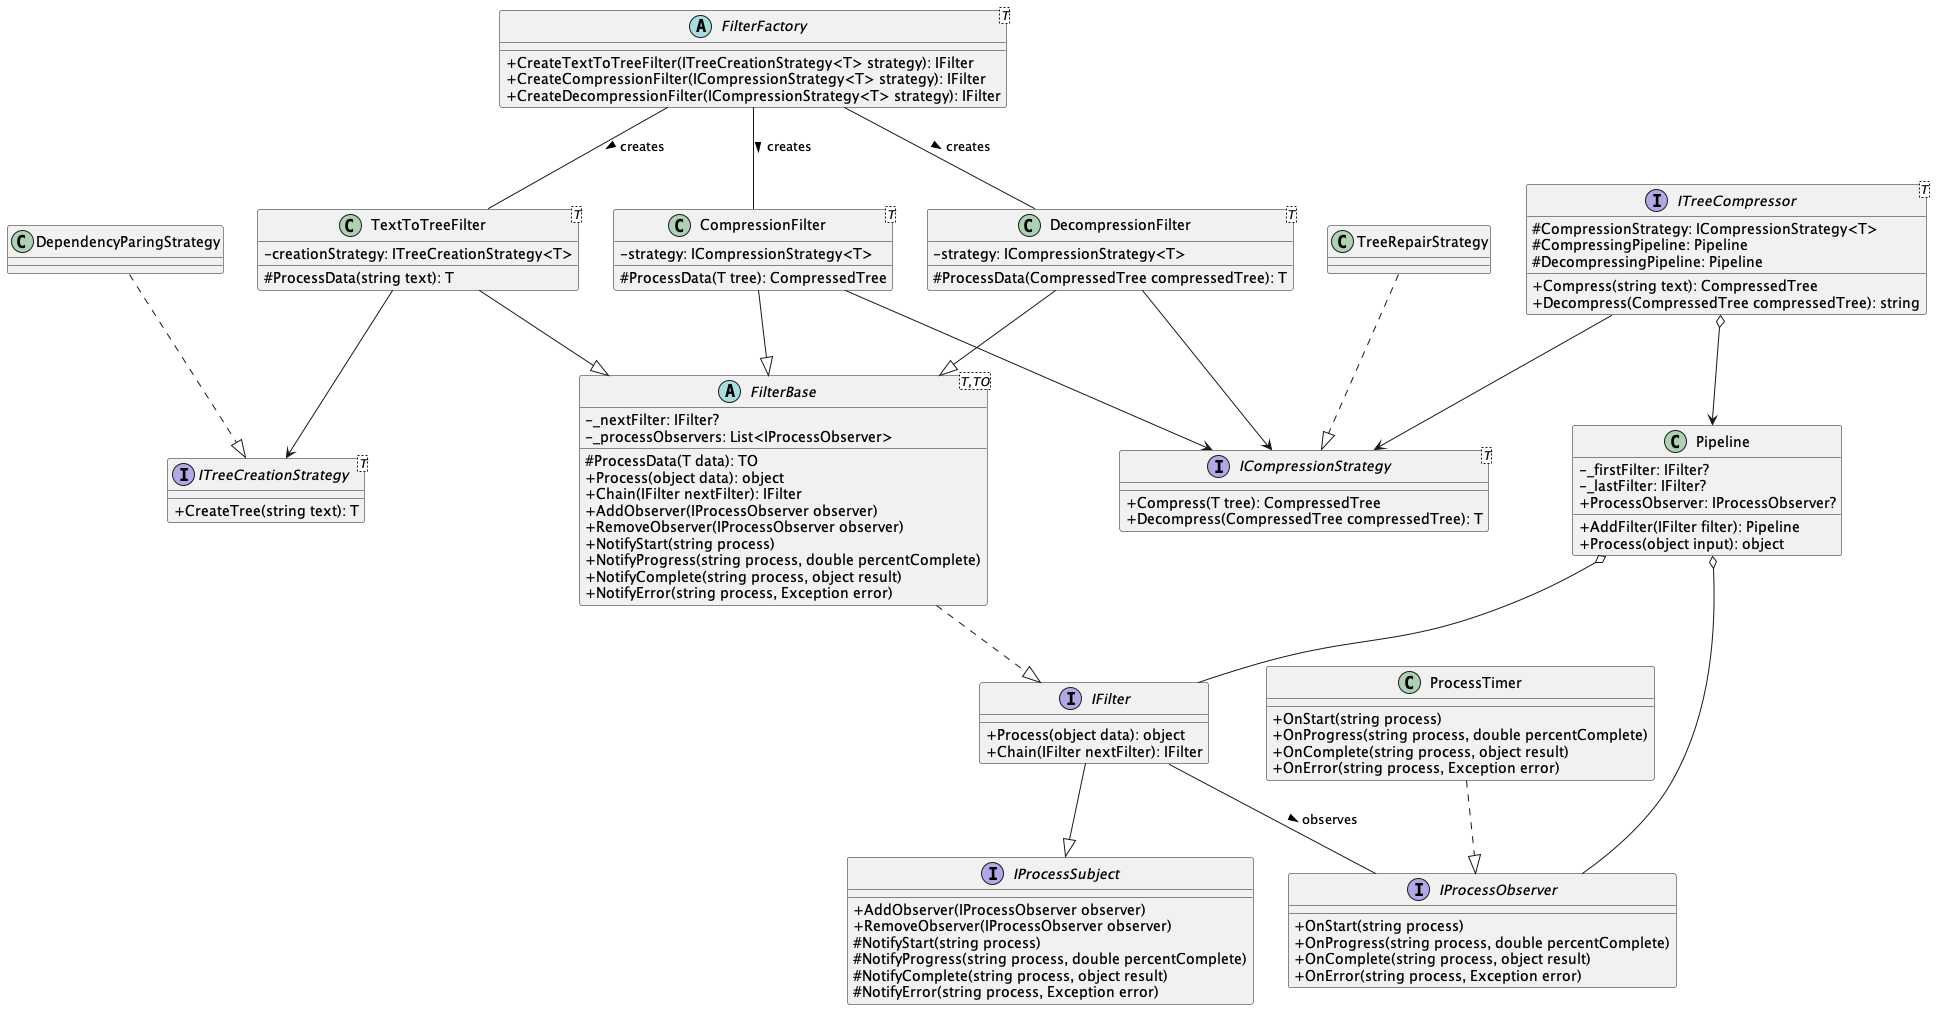
\includegraphics[width=\textwidth]{fig/class-diagram.png}
        \caption{Třídní diagram části implementace zaměření na řetězení filtrů}
        \label{fig:class-diagram}
    \end{figure}
    
\end{frame}

\end{document}